\documentclass[11pt,a4paper,roman]{moderncv}        

\moderncvstyle{banking}                            % style options are 'casual' (default), 'classic', 'oldstyle' and 'banking'
\moderncvcolor{blue}                                % color options 'blue' (default), 'orange', 'green', 'red', 'purple', 'grey' and 'black'
%\renewcommand{\familydefault}{\sfdefault}         % to set the default font; use '\sfdefault' for the default sans serif font, '\rmdefault' for the default roman one, or any tex font name
\nopagenumbers{}                                  % uncomment to suppress automatic page numbering for CVs longer than one page

% character encoding
\usepackage[utf8]{inputenc}
\usepackage{fontawesome}
\usepackage{fontspec}
\usepackage{tabularx}
\usepackage{ragged2e}
% if you are not using xelatex ou lualatex, replace by the encoding you are using
%\usepackage{CJKutf8}                              % if you need to use CJK to typeset your resume in Chinese, Japanese or Korean

% adjust the page margins
\usepackage[scale=0.8]{geometry}
\usepackage{graphicx}
\usepackage{multicol}
%\setlength{\hintscolumnwidth}{3cm}                % if you want to change the width of the column with the dates
%\setlength{\makecvtitlenamewidth}{10cm}           % for the 'classic' style, if you want to force the width allocated to your name and avoid line breaks. be careful though, the length is normally calculated to avoid any overlap with your personal info; use this at your own typographical risks...

\usepackage{import}

% personal data
\name{Masum}{Billal}
%\address{500 College Ave, Swarthmore, PA 19081 }{}{}% optional, remove / comment the line if not wanted; the "postcode city" and and "country" arguments can be omitted or provided empty
\phone[mobile]{+880-1779788023}                   % optional, remove / comment the line if not wanted
% \phone[fixed]{01234 123456}                    % optional, remove / comment the line if not wanted
%\phone[fax]{+3~(456)~789~012}                      % optional, remove / comment the line if not wanted
% \email{xpan1@swarthmore.edu}                               % optional, remove / comment the line if not wanted
% \homepage{shawnpan.me}                         % optional, remove / comment the line if not wanted
% \extrainfo{}                 % optional, remove / comment the line if not wanted
\photo[64pt][0.4pt]{pp1}                       % optional, remove / comment the line if not wanted; '64pt' is the height the picture must be resized to, 0.4pt is the thickness of the frame around it (put it to 0pt for no frame) and 'picture' is the name of the picture file
%\quote{Some quote}                                 % optional, remove / comment the line if not wanted

% to show numerical labels in the bibliography (default is to show no labels); only useful if you make citations in your resume
%\makeatletter
%\renewcommand*{\bibliographyitemlabel}{\@biblabel{\arabic{enumiv}}}
%\makeatother
%\renewcommand*{\bibliographyitemlabel}{[\arabic{enumiv}]}% CONSIDER REPLACING THE ABOVE BY THIS

% bibliography with mutiple entries
%\usepackage{multibib}
%\newcites{book,misc}{{Books},{Others}}
  
\newcommand*{\customcventry}[7][.25em]{
  \begin{tabular}{@{}l} 
    {\bfseries #4}
  \end{tabular}
  \hfill% move it to the right
  \begin{tabular}{l@{}}
     {\bfseries #5}
  \end{tabular} \\
  \begin{tabular}{@{}l} 
    {\itshape #3}
  \end{tabular}
  \hfill% move it to the right
  \begin{tabular}{l@{}}
     {\itshape #2}
  \end{tabular}
  \ifx&#7&%
  \else{\\%
    \begin{minipage}{\maincolumnwidth}%
      \small#7%
    \end{minipage}}\fi%
  \par\addvspace{#1}}

\newcommand{\SubItem}[1]{
	{\setlength\itemindent{15pt} \item[-] #1}
}


\newcommand*{\customcvproject}[4][.25em]{
%   \vfill\noindent
  \begin{tabular}{@{}l} 
    {\bfseries #2}
  \end{tabular}
  \hfill% move it to the right
  \begin{tabular}{l@{}}
     {\itshape #3}
  \end{tabular}
  \ifx&#4&%
  \else{\\%
    \begin{minipage}{\maincolumnwidth}%
      \small#4%
    \end{minipage}}\fi%
  \par\addvspace{#1}}

\setlength{\tabcolsep}{12pt}

%----------------------------------------------------------------------------------
%            content
%----------------------------------------------------------------------------------
\begin{document}
%\begin{CJK*}{UTF8}{gbsn}                          % to typeset your resume in Chinese using CJK
%-----       resume       ---------------------------------------------------------

\makecvtitle
\vspace{-.2in}
\begin{center}
	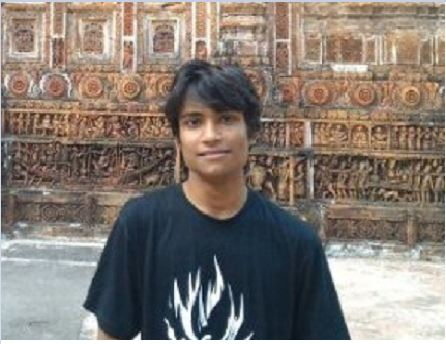
\includegraphics[scale=.2]{pp1}
\end{center}
\vspace*{-.2in}

\section{EDUCATION}
{\customcventry{BSC}{CSE}{University of Dhaka}{Dhaka, Bangladesh}{}{}}


\section{EXPERIENCE}
{\customcventry{October 2018 - May 2019}{Machine learning engineer}{Auleek}{Dhaka, Bangladesh}{}
{\begin{itemize}
  \item \textbf{Hestia}
  \SubItem{Used deep learning in tensorflow to extract features (door, wall, window etc) from floorplan images.}
  \SubItem{RnD on interior design automation, such as structural groups of furnitures and finding the most optimal configuration.}
  \SubItem{Implemented mesh generation for different kind of object shapes, mesh combining such as union or intersection, checking if an object can be placed in an arrangement.}
\end{itemize}
}

{\customcventry{March 2017 - September 2018}{Software Engineer}{Reve Systems}{Dhaka, Bangladesh}{}
{\begin{itemize}
  \item \textbf{e-Veterinary Services}
  \SubItem{Worked full-stack from Spring Boot framework to thymeleaf frontend templating, bootstrap and javascript.}
  \SubItem{Used JPA for hibernate-like ORM manipulation.}
  \SubItem{Followed agile development process for meeting tight deadline.}
  \SubItem{Live server of project: \texttt{http://evet.gov.bd/login}}
  \item \textbf{IP Log}
  \SubItem{Worked on networking and socket protocols for receiving and processing all incoming and outgoing packets in a network.}
  \SubItem{Used multi threading for avoiding packet loss and prevented buffer overflow during packet receiving.}
  \item \textbf{Surveillance}
  \SubItem{Worked on backend of this Struts based project.}
  \SubItem{Implemented features such as duplicate number detection, home or office detection etc based on geolocation.}
  \SubItem{Did RnD on geolocation, 2G/3G/GSM protocols and distance estimation models from signal strength and related parameters.}
  \SubItem{Implemented trilateration as part of this project.}
\end{itemize}
}

{\customcventry{April 2016-September 2016}{Software developer and data analyst}{Threat Equation PTE LTD.}{Dhaka, Bangladesh}{Remote job}
{\begin{itemize}
  \item \textbf{Threat Equation}
  \SubItem{Worked on backend of a Django dashboard.}
  \SubItem{Pared server logs for feeding data into the learning model for predicting vulnerability in the application.}
  \SubItem{Used libraries such as Chart.js to show visualization of predicted results and related data in dashboard.}
\end{itemize}
}

\section{Achievements and voluntary experience}
{
	\cvitem{2009}{Medal in regional mathematical olympiad, Dhaka, Bangladesh.}
	\cvitem{2010}{Medal in regional and national mathematical olympiad, Bangladesh.}
	\cvitem{2011-2015}{Trainer (specially for number theory) in national and IMO math camps.}
	\cvitem{2012}{Participated in Dhaka regional ICPC, rank 18.}
	\cvitem{2012}{Participated in Inter-University Programming Contest, Islamic University of Technology, Bangladesh, rank 13.}
	\cvitem{2013}{Participated in Dhaka regional ICPC, rank 17.}
	\cvitem{2013}{Participated in Inter-University Programming Contest, North South University, Bangladesh, rank 9.}
}

\section{Publications}
\cvitemwithcomment{2019}{Topics in Number Theory: An Olympiad Oriented Approach}{Masum Billal, Amir Hossein}
\cvitemwithcomment{2015}{Similarity Aggregation for Collaborative Filtering, AIST Conference}{Sheikh Muhammad Sarwar, Masum Billal, Mahmudul Hasan, Dimitry I. Ignatov}
\cvitemwithcomment{2014}{A Nice Theorem in Multiplicative Functions, Issue 63, Eureka, Cambridge Mathematical Society}{Masum Billal}
\cvitemwithcomment{2012}{Exponent GCD Lemma, Issue 6, Mathematical Reflections}{Masum Billal}

\section{PROJECTS}
{\customcvproject{Localizer}{2019}
{\begin{itemize}
  \item A self-contained tool for localizing objects in images.
  \item Used darkflow to implement state-of-the-art YOLO algorithm for object detection in tensorflow.
\end{itemize}
}

{\customcvproject{Improving Collaborative Filtering Based Recommender Systems}{BSc Thesis, 2016}
{\begin{itemize}
  \item Developed a new recommender system.
  \item Achieved F-1 score of almost 75\% on movielens dataset.
  \item Introduced, implemented ideas of aggregating multiple metrics and tested the hypothesis.
  \item Currently work on progress to improve it even further.
\end{itemize}
}
}

{
	\customcvproject{Otaku Store}{2016}
	{\begin{itemize}
			\item Worked full stack for building a Django framework based e-commerce site.
	\end{itemize}}
}

{\customcvproject{A Recommender System}{2016}
	{\begin{itemize}
			\item Developed a recommender system based on Multinomial Naive Bayes for learning purpose.
		\end{itemize}
	}
}
\section{Others}
\cvitem{Github}{\texttt{https://github.com/fifaboy}}
\cvitem{LinkedIn}{\texttt{https://www.linkedin.com/in/billalmasum93/}}
\cvitem{Blog}{\texttt{https://karushib.wordpress.com/}}
\end{document}
